\section{Problem 3-1}
\label{sec:problem1}

\subsection*{(a) System of six first-order differential equations}

The two-body differential equation (Eq.~1.15) is
\begin{equation}
    \ivect{a} + \frac{\mu}{r^3}\vect{r} = \vect{0}.
\end{equation}
This equation is second order in position. Treating the inertial velocity as a second unknown turns it into two first-order vector equations:
\begin{equation}
    \dot{\vect{r}} = \ivect{v}, \qquad
    {}^{I}\dot{\underline{v}} = -\frac{\mu}{r^3}\,\vect{r}.
    \label{eq:p1-firstorder}
\end{equation}
Both unknown vectors can be broken down into their PCI components:
\begin{equation}
    [\vect{r}]_I = \begin{bmatrix} x \\ y \\ z \end{bmatrix}, \qquad
    \big[\ivect{v}\big]_I = \begin{bmatrix} v_x \\ v_y \\ v_z \end{bmatrix}, \qquad
    r = \sqrt{x^2 + y^2 + z^2}.
\end{equation}
Thus, we can obtain six first-order differential equations from the PCI components:
\begin{equation}
    \begin{aligned}
        \dot{x}  &= v_x, &\qquad \dot{v}_x &= -\frac{\mu}{r^3}\,x, \\
        \dot{y}  &= v_y, &\qquad \dot{v}_y &= -\frac{\mu}{r^3}\,y, \\
        \dot{z}  &= v_z, &\qquad \dot{v}_z &= -\frac{\mu}{r^3}\,z.
    \end{aligned}
\end{equation}
Collecting the six unknowns into one state vector, the system is
\begin{equation}
    \vect{p} = \begin{bmatrix} x \\ y \\ z \\ v_x \\ v_y \\ v_z \end{bmatrix}, \qquad
    \dot{\vect{p}} = \begin{bmatrix} v_x \\ v_y \\ v_z \\ -\mu x / r^3 \\ -\mu y / r^3 \\ -\mu z / r^3 \end{bmatrix}.
    \label{eq:p1-pdot}
\end{equation} 

\subsection*{(b) Right-hand side function}
 
File \texttt{twobody.py} implements Eq.~\eqref{eq:p1-pdot} as \texttt{two\_body\_ode(t, p, mu)}. It splits \texttt{p} into position (\texttt{p[0:3]}) and velocity (\texttt{p[3:6]}), computes the PCI acceleration, and returns the two as \texttt{pdot}.

\subsection*{(c) Integration}

The function \texttt{propagate\_two\_body} builds the initial state from the given position and velocity and integrates \texttt{two\_body\_ode} from $t_0$ to $t_f$ using \texttt{solve\_ivp} with method \texttt{DOP853} (a variale-step integrator similar to MATLAB's \texttt{ode113}). Both the relative and absolute tolerances are set to $10^{-12}$.

\vspace{1pt}

\paragraph{Choice of tolerances.}
The value $10^{-12}$ follows a study of integrator tolerances for orbit propagation by Rocha (2018), which recommends a relative tolerance of at least $10^{-10}$ for Earth orbits, with $10^{-12}$ being preferable \cite[p.~22]{rocha2018}.

\subsection*{(d) Results}

The resulting PCI position and inertial velocity at $t=t_f$ for the six given cases, along with the integrated trajectories, are shown below.

\programoutput{outputs/problem1.txt}

\begin{figure}[H]
    \centering
    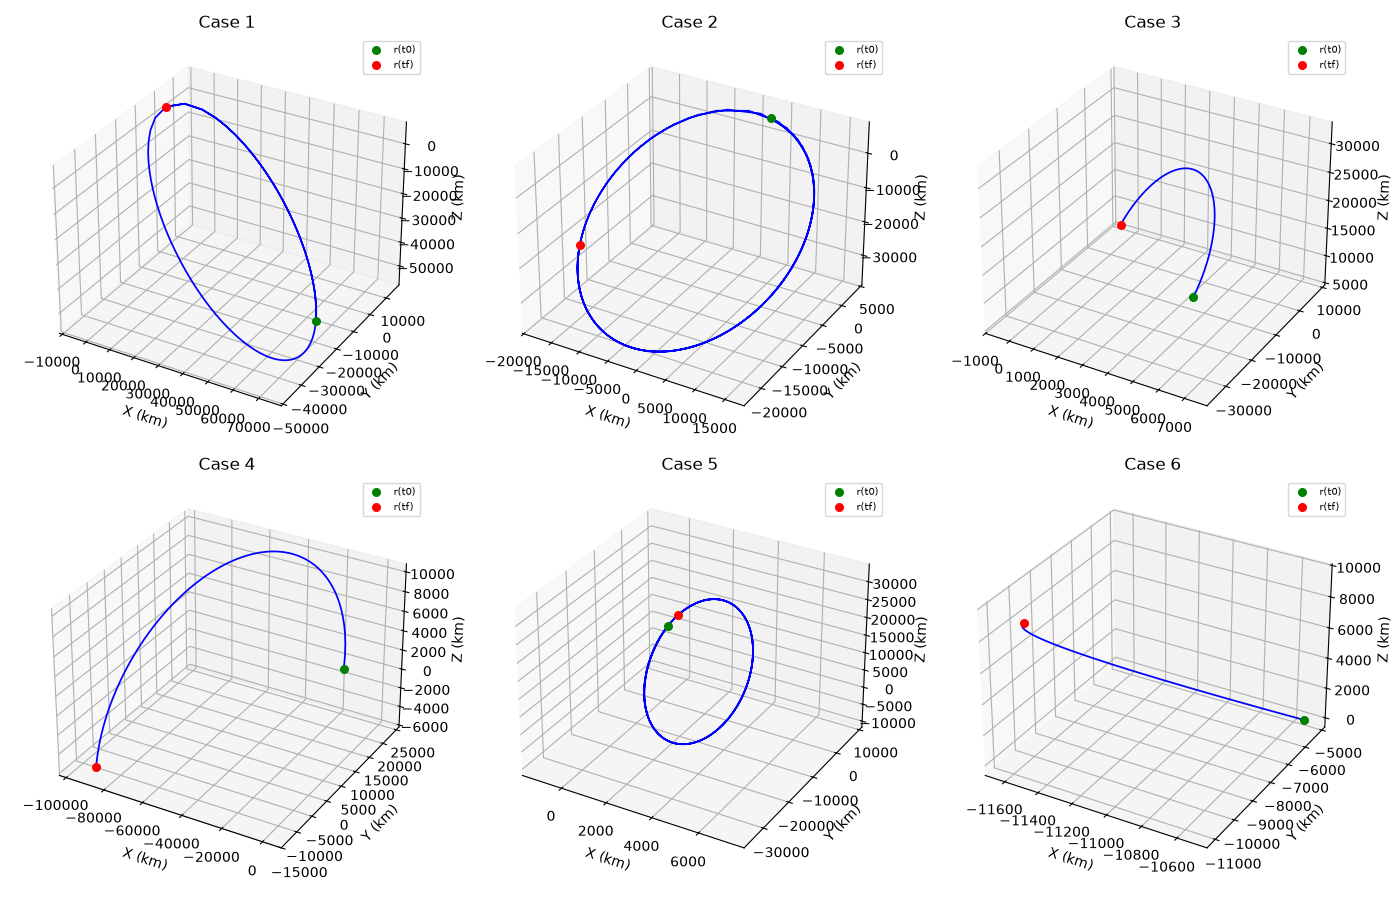
\includegraphics[width=\textwidth]{figures/problem1_orbits.png}
    \caption{PCI position trajectories, $[\vect{r}]_I$, for the six cases of Problem 1, obtained by integrating the two-body ODE from $t_0$ to $t_f$.}
\end{figure}

\FloatBarrier
